\documentclass{article}
\usepackage{polski}
\usepackage[top=2cm,bottom=2.5cm,left=2cm,right=2cm]{geometry}
\usepackage{graphicx}
\usepackage{float}
\usepackage[colorlinks=true, allcolors=blue]{hyperref}

\begin{document}
\title{\Huge Projekt z Baz Danych \\Dokumentacja}
\author{\LARGE Wojciech Kowal, Mateusz Łazowy, Darina Khamrakulova, Jakub Idasiak}
\date{\Large Styczeń 2026}
\maketitle
\Large
\tableofcontents
\newpage
\section{\LARGE Wstęp}
Dokumentacja ma za zadanie przedstawić aspekty projektu z Baz Danych. Projekt miał na celu stworzenie, wypełnienie, przeanalizowanie i stworzenie raportu z bazy danych do nowoczesnego parku rozrywki AiBtcQuantLandia. Baza zawiera m.in informacje o pracownikach, atrakcjach, awariach, gościach i ich wizytach, transkacjach, biletach, zdarzeniach i ubezpieczeniach od nich.
\section{\LARGE Spis użytych technologii}
Do projektu użyto następujących technologii:
\begin{itemize}
    \item ERD Editor v2.1.0 - stworzenie schematu bazy danych.
    \item Biblioteki Pythona:
    \begin{enumerate}
        \item random - generowanie liczb losowych
        \item datetime - daty
        \item decimal - w celu otrzymywania wyniku z odpowiednią ilością cyfr po przecinku
        \item mysql.connector - komunikacja Pythona z bazą
        \item pandas - przetwarzanie i analiza danych
        \item numpy - obliczenia numeryczne
        \item matplotlib - wizualizacja
        \item seaborn - rozszerzenie wizualizacji
    \end{enumerate}
    \item R:
    \newline
    R markdown - format pliku obsługujący kod i tekst
    \newline
    Pakiety:
    \begin{enumerate}
        \item knitr - generowanie raportów
        \item reticulate - integracja R z Pythonem
    \end{enumerate}
    \item LaTeX - przygotowanie dokumentacji projektu
\end{itemize}
\section{\LARGE Spis plików}
\begin{itemize}
    \item dokumentacja - katalog zawierający:
    \begin{enumerate}
        \item dokumentacja.tex - kod źródłowy LaTeXa generujący dokumentację
        \item schemat\textunderscore bazy.png - plik png zawierający schemat bazy danych
        \item dokumentacja.pdf - dokumentacja w formacie pdf
    \end{enumerate}
    \item schemat.sql - schemat bazy danych w formacie sql, pozwalający na stworzenie bazy danych
    \item generowanie\textunderscore danych.py - skrypt generujący i wstawiający dane do bazy danych
    \item analiza.py - program zawierający analizę danych.
    \item baza\textunderscore schemat.vuerd - schemat bazy danych w formacie vuerd
    \item raport - katalog zawierający:
    \begin{enumerate}
        \item raportAUTO.Rmd - kod źródłowy R generujący raport
        \item raportAUTO.pdf - raport w formacie pdf
        \item raportLADNY.pdf - nie dynamiczna wersja raportu zawierająca wyciąganie wniosków
    \end{enumerate}
\end{itemize}
\section{\LARGE Kolejność i sposób uruchamiania plików}
Projekt był testowany na Pythonie 3.12, R 4.5. wymaga również LaTeXa i środowisk umożliwiająych włączanie i kompilacje plików, oraz zainstalowanych bibliotek z Spisu użytych technologii.
Do wyboru mamy następujące możliwości:
\begin{enumerate}
\item Jeśli chcemy jedynie zobaczyć raport, to uruchamiamy raportAUTO.pdf
\item Jeśli chcemy wygenerować nowe dane i nowy raport to uruchamiamy:
\begin{itemize}
    \item generowanie\textunderscore danych.py
    \item raportAUTO.Rmd
\end{itemize}
\item Jeśli chcemy odtworzyć projekt na własnej bazie danych to:
\begin{itemize}
    \item Tworzymy pustą bazę
    \item używamy schemat.sql
    \item zmieniamy w generowanie\textunderscore danych.py oraz raportAUTO.Rmd dane połączenia na dane naszej bazy
    \item wykonujemy 2.
\end{itemize}
\end{enumerate}
\section{\LARGE Schemat bazy danych}
\begin{figure}[H]
    \centering
    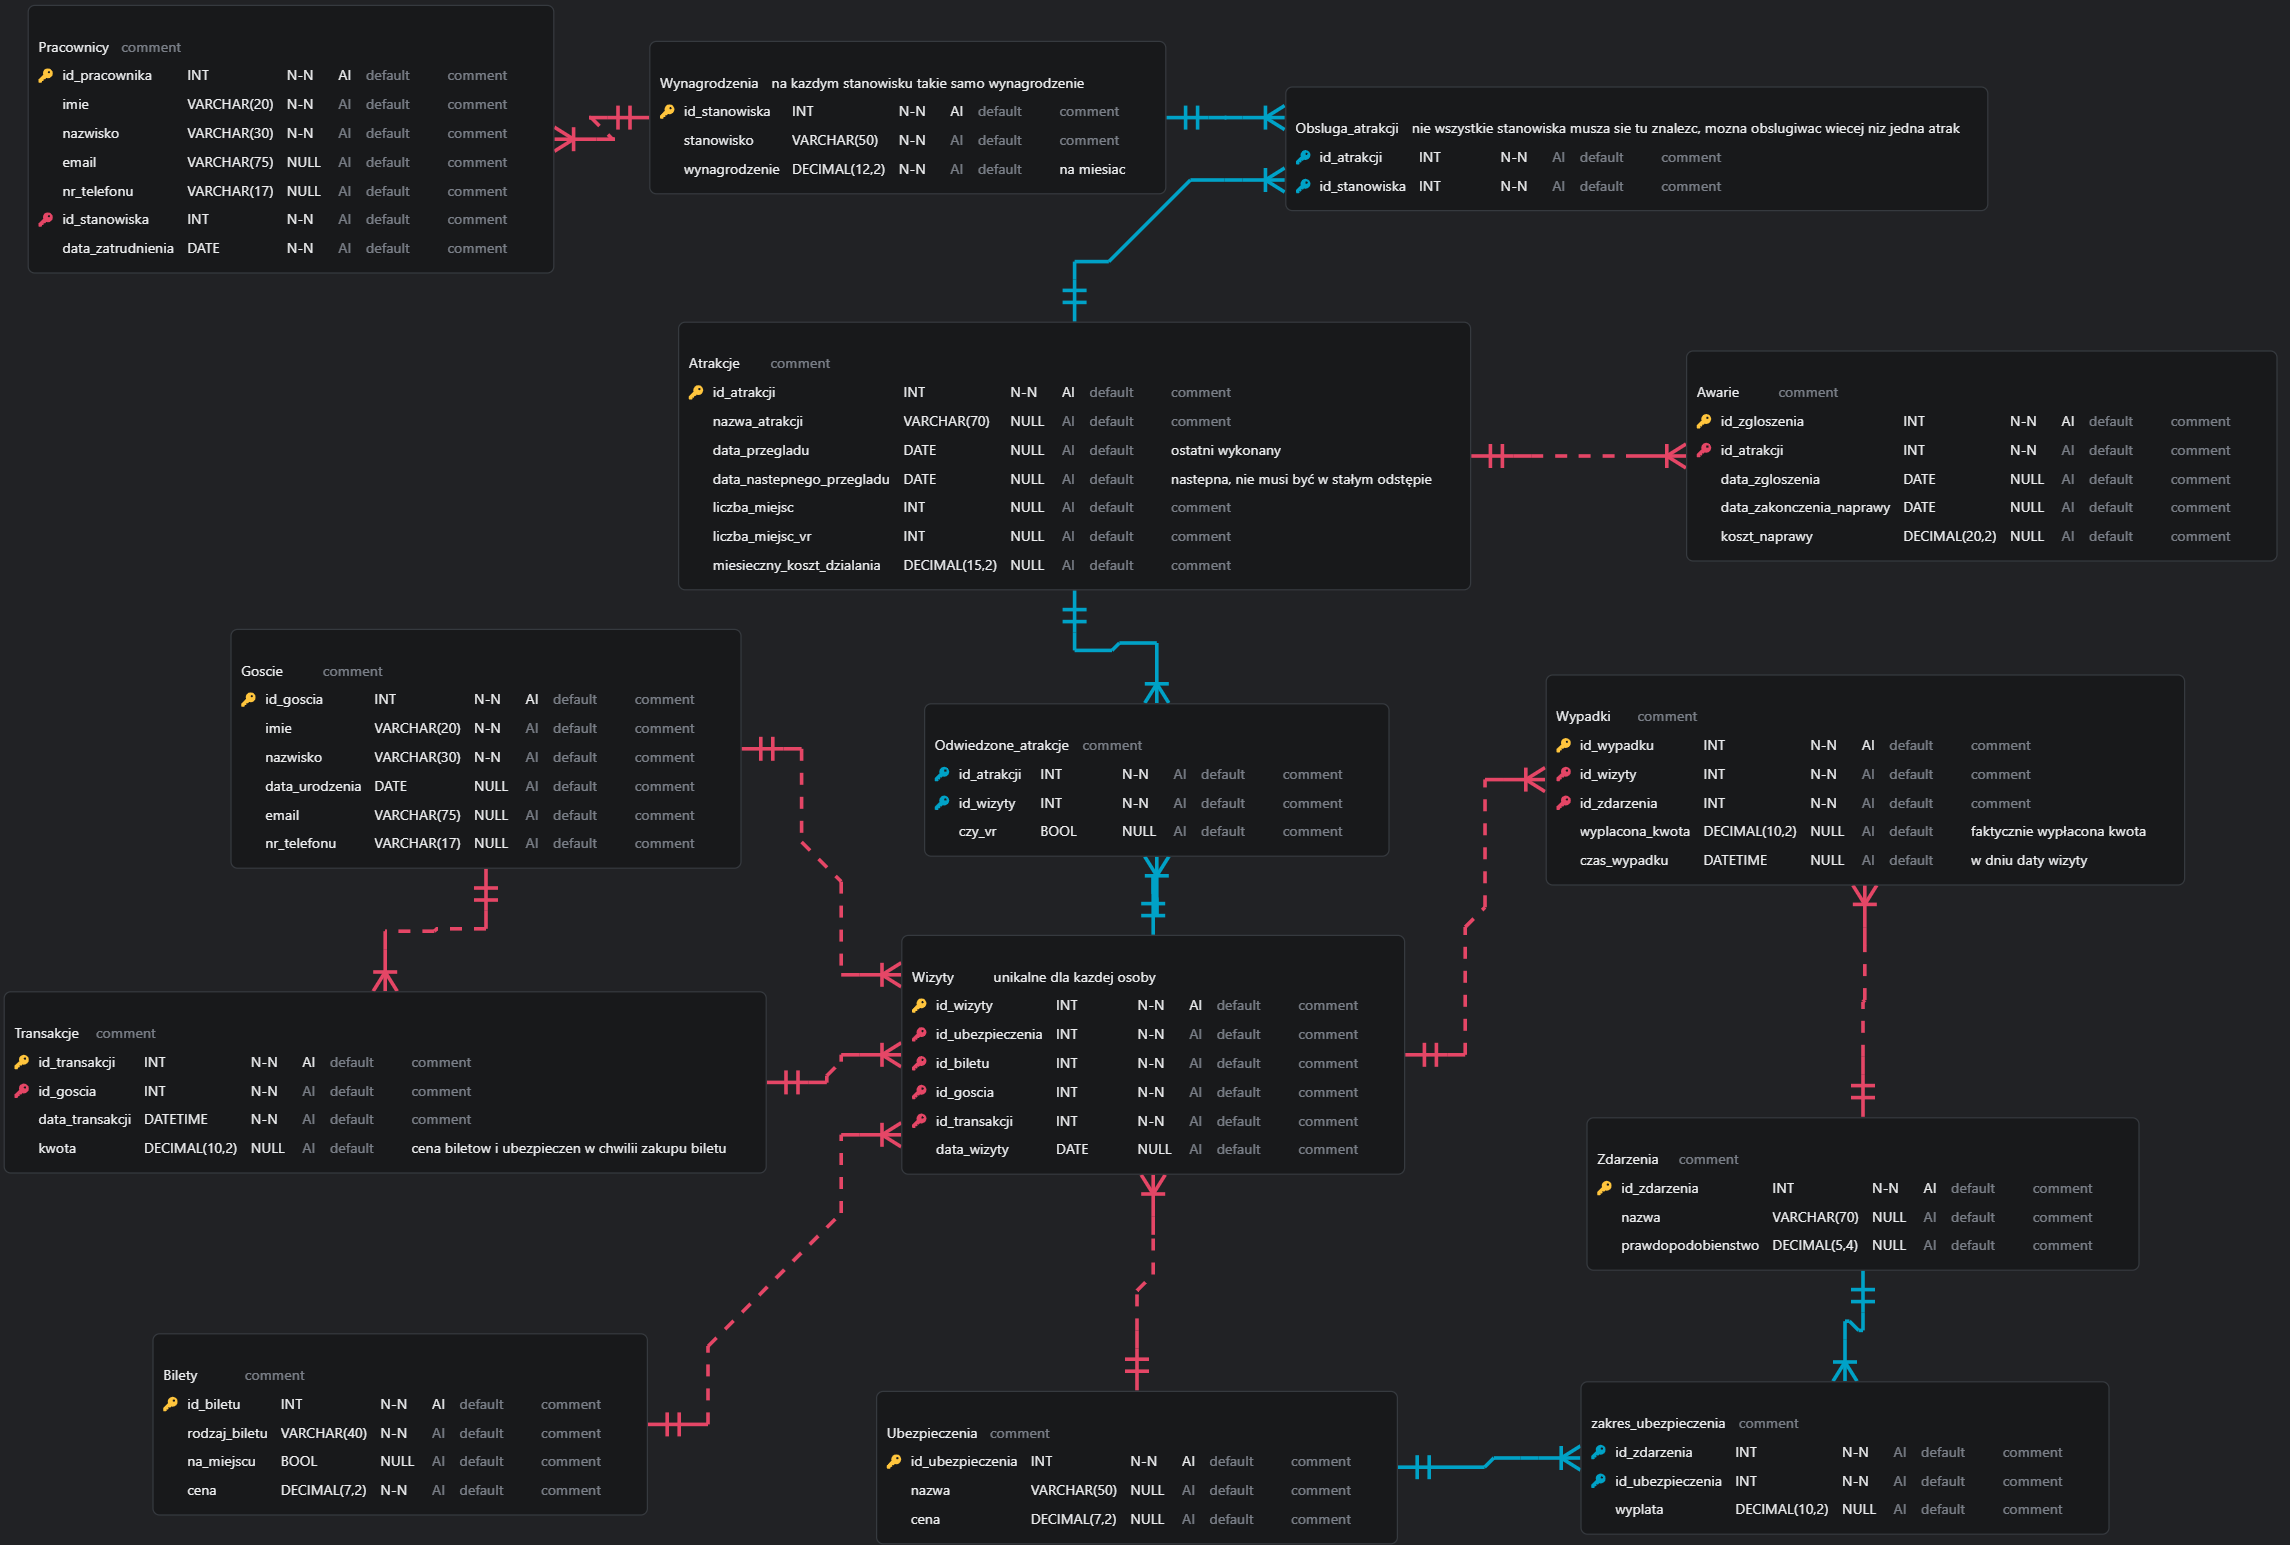
\includegraphics[width = \textwidth]{schemat_bazy.png}
    \caption{\normalsize Schemat bazy danych}
\end{figure}
\subsection{Relacje między tabelami}
\begin{itemize}
    \item Wynagrodzenia z Pracownicy - relacja 1:n, Pracownicy mogą mieć takie same stanowiska.
    \item Atrakcje i Wynagordznia z Obsluga-atrakcji - relacje 1:n, do atrakcji może być przypisane wiele stanowisk, ale też stanowisko może nie byc przypisane do atrakcji.
    \item Atrakcje z Awarie - relacja 1:n, atrakcja może mieć wiele awarii.
    \item Goscie z Transakcje - relacja 1:n, gość może wykonać wiele transakcji.
    \item Zdarzenia i Ubezpieczenia z zakres\textunderscore ubezpieczenia - relacje 1:n, różne ubezpieczenia mogą mieć różne wypłaty dla tych samych zdarzeń.
    \item Goscie, Transakcje, Bilety i Ubezpieczenia z Wizyty - relacje 1:n, gość może odbyć wiele wizyt, podczas 1 transakcji można kupić bilety na więcej wizyt, typy biletów nie są unikalne - każdy używa jednego z istniejących, tak samo z ubezpieczeniami.
    \item Wizyty i Atrakcje z Odwiedzone\textunderscore atrakcje - relacje 1:n, podczas wizyty można odwiedzić wiele atrakcji.
    \item Wizyty z zdarzenia - relacje 1:n, podczas wizyty może wydarzyć się więcej niż jedno zdarzenie, zdarzenia wśród różnych gości są powtarzalne.
\end{itemize}
\section{\LARGE Lista zależności funkcyjnych}
\begin{enumerate}
\item Pracownicy 
\begin{itemize}
    \item Zależność funkcyjna: \newline
    (id\textunderscore pracownika) $\rightarrow$ (imie, nazwisko, email, nr\textunderscore telefonu, id\textunderscore stanowiska, data\textunderscore zatrudnienia)
    \item Wyjaśnienie: \newline
    Klucz główny jednoznacznie identyfikuje dane osobowe pracownika, oraz jego stanowisko będące kluczem obcym.
\end{itemize}
\item Wynagrodzenia
\begin{itemize}
    \item Zależność funkcyjna: \newline
    (id\textunderscore stanowiska) $\rightarrow$ (stanowisko, wynagrodzenie)
    \item Wyjaśnienie: \newline
    Klucz główny jednoznacznie identyfikuje stanowisko oraz jego wynagrodzenie.
\end{itemize}
\item Atrakcje 
\begin{itemize}
    \item Zależność funkcyjna: \newline
    (id\textunderscore atrakcji) $\rightarrow$ (nazwa\textunderscore atrakcji, data\textunderscore przegladu, data\textunderscore nastepnego\textunderscore przegladu, liczba\textunderscore miejsc, liczba\textunderscore miejsc\textunderscore vr, miesieczny\textunderscore koszt\textunderscore dzialania)
    \item Wyjaśnienie: \newline
    Klucz główny jednoznacznie identyfikuje dane o atrakcjach.
\end{itemize}
\item Obsluga\textunderscore atrakcji 
\begin{itemize}
    \item Zależność funkcyjna: \newline
    (id\textunderscore stanowiska, id\textunderscore atrakcji) $\rightarrow$ $\emptyset$
    \item Wyjaśnienie: \newline
    Tabela składa się z samego klucza głównego, który składa się z kluczy obcych.
\end{itemize}
\item Awarie 
\begin{itemize}
    \item Zależność funkcyjna: \newline
    (id\textunderscore zgloszenia) $\rightarrow$ (id\textunderscore atrakcji, data\textunderscore zgloszenia, data\textunderscore zakonczenia\textunderscore naprawy, koszt\textunderscore naprawy)
    \item Wyjaśnienie: \newline
    Klucz główny jednoznacznie identyfikuje informacje na temat awarii oraz atrakcji, której się ta przydarzyła (klucz obcy).
\end{itemize}
\item Goscie 
\begin{itemize}
    \item Zależność funkcyjna: \newline
    (id\textunderscore goscia) $\rightarrow$ (imie, nazwisko, data\textunderscore urodzenia, email, nr\textunderscore telefonu)
    \item Wyjaśnienie: \newline
    Klucz główny jednoznacznie identyfikuje dane osobowe gościa.
\end{itemize}
\item Transakcje 
\begin{itemize}
    \item Zależność funkcyjna: \newline
    (id\textunderscore transakcji) $\rightarrow$ (id\textunderscore goscia, data\textunderscore transakcji, kwota)
    \item Wyjaśnienie: \newline
    Klucz główny jednoznacznie identyfikuje dane transakcji, oraz gościa, który wykonał transakcje (klucz obcy).
\end{itemize}
\item Zdarzenia
\begin{itemize}
    \item Zależność funkcyjna: \newline
    (id\textunderscore zdarzenia) $\rightarrow$ (nazwa, prawdopodobienstwo)
    \item Wyjaśnienie: \newline
    Klucz główny jednoznacznie identyfikuje zdarzenie i jego prawdopodobieństwo wydarzenia.
\end{itemize}
\item Ubezpieczenia
\begin{itemize}
    \item Zależność funkcyjna: \newline
    (id\textunderscore ubezpieczenia) $\rightarrow$ (nazwa, cena)
    \item Wyjaśnienie: \newline
    Klucz główny jednoznacznie identyfikuje nazwę i cenę ubezpieczenia.
\end{itemize}
\item zakres\textunderscore ubezpieczenia 
\begin{itemize}
    \item Zależność funkcyjna: \newline
    (id\textunderscore zdarzenia, id\textunderscore ubezpieczenia) $\rightarrow$ (wyplata)
    \item Wyjaśnienie: \newline
    Klucz główny składający się z kluczy obcych jednoznacznie identyfikuje wypłacaną kwotę dla danego zdarzenia w danym ubezpieczeniu.
\end{itemize}
\item Bilety 
\begin{itemize}
    \item Zależność funkcyjna: \newline
    (id\textunderscore biletu) $\rightarrow$ (rodzaj\textunderscore biletu, na\textunderscore miejscu, cena)
    \item Wyjaśnienie: \newline
    Klucz główny jednoznacznie identyfikuje rodzaj biletu, jego cenę oraz to czy jest na miejscu.
\end{itemize}
\item Wizyty 
\begin{itemize}
    \item Zależność funkcyjna: \newline
    (id\textunderscore wizyty) $\rightarrow$ (id\textunderscore ubezpieczenia, id\textunderscore biletu, id\textunderscore goscia, id\textunderscore transakcji, data\textunderscore wizyty)
    \item Wyjaśnienie: \newline
    Klucz główny jednoznacznie identyfikuje datę wizyty, oraz gościa (klucz obcy), ubezpieczenie które posiada (klucz obcy), bilet (klucz obcy), transakcje związaną z wizytą (klucz obcy).
\end{itemize}
\item  Odwiedzone\textunderscore atrakcje
\begin{itemize}
    \item Zależność funkcyjna: \newline
    (id\textunderscore atrakcji, id\textunderscore wizyty) $\rightarrow$ (czy\textunderscore vr)
    \item Wyjaśnienie: \newline
    Klucz główny który jest kluczami obcymi jednoznacznie identyfikuje odwiedzenie atrakcji oraz to czy odbyło się ono za pomocą vr.
\end{itemize}
\item Wypadki 
\begin{itemize}
    \item Zależność funkcyjna: \newline
    (id\textunderscore wypadku) $\rightarrow$ (id\textunderscore wizyty, id\textunderscore zdarzenia, wyplacona\textunderscore kwota, czas\textunderscore wypadku)
    \item Wyjaśnienie: \newline
    Klucz główny jednoznacznie identyfikuje to podczas jakiej wizyty (klucz obcy), jakie zdarzenie (klucz obcy) wydarzyło się kiedy i faktycznie wypłaconą kwotę.
\end{itemize}
\end{enumerate}
\section{\LARGE Uzasadnienie, że baza jest w EKNF}
Baza danych jest w EKNF, ponieważ
\begin{enumerate}
    \item Spełnia założenia 1NF - wiersze się nie powtarzają, oraz atrybuty są elementarne (atomowe, niepodzielne).
    \item Spełnia założenia 2NF - Wszystkie atrybuty niekluczowe są w pełni zależne funkcyjnie od całego klucza głównego.
    \item Spełnia założenia 3NF - atrybuty niekluczowe nie są zależne funkcyjnie od innych atrybutów niekluczowych, nie ma zależności przechodnich.
    \item Spełnia założenia EKNF - każda nietrywialna zależność funkcyjna zaczyna się od nadklucza, albo kończy się na atrybucie elementarnym.
\end{enumerate}
\section{\LARGE Podsumowanie i trudności}
\begin{itemize}
    \item Trudności w realizacji projektu:
    \begin{enumerate}
        \item Zrozumienie normalizacji baz danych, zwłaszcza różnicy między 3NF, EKNF a BCNF.
        \item Stworzenie sensownej bazy danych zawierających odpowiednie kolumny i tabele.
        \item Generowanie rozsądnych danych, takich żeby nie były sprzeczne, zwłaszcza w przypadku dat oraz czasochłonność tej części.
        \item W przypadku Analizy Danych - zrozumienie bazy, typów danych, tego jak wyciągnąć poszczególne informacje.
    \end{enumerate}
    \item Podsumowanie \newline
    Projekt był wymagający i nie raz wymagał douczenia się teorii baz danych, Pythona czy R, jednak dzięki temu rozwinęliśmy swoje umiejętności w tych obszarach. Projekt również wymagał pracy grupowej, zorganizowania, podziału obowiązków i efektywnej współpracy co w przyszłości będzie przydatne w pracy zawodowej.
\end{itemize}

\end{document}
